\newpage
\noindent
\textbf{Beispiel 3}\\ \\
a)\\ \\
Freigeschnittene Körper:
\begin{figure}[h]
	\centering
	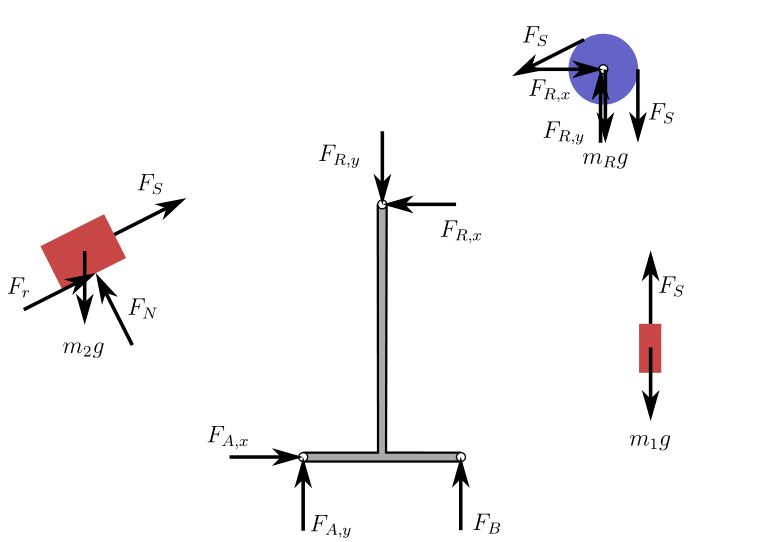
\includegraphics[width=10cm]{tikz/07_02_2020_3a}
\end{figure}
\newline
b)\\ \\
Aus der Zeichnung folgt für die Seilkraft
\[
	F_S = m_1g
\]
c) \\ \\
Mit den Gleichgewichtsbedingungen für die Masse 2 der und der Haftreibung, darf die Masse 2 den Wert
\[
	m_{2,max} = \frac{m_1}{\mu_H \cos(\alpha)}
\]
d) \\ \\
Um die Lagerkräfte zu bestimmen müssen zuerst die Gleichgewichtsbedingungen für die Lager bestimmt werden. Durch Umformen erhält man schließlich die Lagerkräfte
\begin{align*}
	F_{R,x} &= m_1g\cos(\alpha) \\
	F_{R,y} &= m_Rg + m_1g(1 + \sin(\alpha))
\end{align*}
e) \\ \\
Analog zu Punkt d) erhält man
\begin{align*}
	F_{A,x} &= m_1g\cos(\alpha) \\
	F_{A,y} &= \frac{1}{2}(m_Rg + m_1g(1 + \sin(\alpha))) + \frac{l_1}{l_2}m_1g\cos(\alpha) \\
	F_B &= \frac{1}{2}(m_Rg + m_1g(1 + \sin(\alpha))) - \frac{l_1}{l_2}m_1g\cos(\alpha)
\end{align*}
\newpage
\noindent
f)\\ \\
Über sämtliche aufgestellten Gleichgewichtsbedingungen erhält man für die maximale Höhe
\[
	l_{1,max} = \frac{l_2(m_R + m_1(1 + \sin(\alpha)))}{2m_1\cos(\alpha)}
\]
g)\\ \\
Aus der Impulsbilanz
\[
	\ddot{s}(m_1 + m_2 + \frac{I_R}{r^2}) = F + m_1g - F_r - mg\sin(\alpha)
\]
erhält man die Bewegungsgleichung
\[
	\ddot{s} = \frac{F + m_1g - F_r - mg\sin(\alpha)
		}{m_1 + m_2 + \frac{I_R}{r^2}}
\]